\documentclass{article}
\usepackage{graphicx}
\usepackage{mathtools}
\DeclareGraphicsExtensions{.pdf,.png,.jpg}

\begin{document}

\title{Bayesian Identity Metric for Genotyping}
\author{Iain Bancarz, ib5@sanger.ac.uk }
\date{May 2016}
\maketitle


\section{Introduction}

This document describes the theoretical background to the Bayesian identity check, which is a QC metric introduced in pipeline release 1.11.5.

An identity check compares calls on a set of QC plex SNPs, between Infinium and another genotyping platform, such as Sequenom and/or Fluidigm. We observe \emph{concordance} between Infinium and the alternate platform on the QC plex, and use it to evaluate \emph{identity}. If concordance is too low, we are not confident that the production and QC calls derive from the same sample; this may indicate a sample swap or poor data quality.

Key questions include:

\begin{itemize}
\item How do we handle no-calls? How many non-null calls are required to evaluate identity?
\item What is an appropriate concordance threshold for sample identity?
\item How do we handle multiple QC plex runs, potentially on different platforms?
\end{itemize}

Previous versions of the identity check set an \textit{ad hoc} threshold on concordance, which was used to mark samples as passing or failing QC. The Bayesian approach seeks to place the identity check on a sound probabilistic footing, in which the underlying assumptions are made explicit.

\section{Bayesian Inference}

Bayesian inference is a widely used statistical method in which we specify \emph{prior} assumptions, and update the probability of an event based on observed data, finding what is known as the \emph{posterior} probability.

This is done using \emph{Bayes' rule}:

\begin{displaymath}
\Pr(H|E) = \frac{\Pr(E|H)\Pr(H)}{\Pr(E)}
\end{displaymath}

where:

\begin{itemize}
\item $H$ is a \emph{hypothesis}; ``samples are identical'' or ``samples are not identical''
\item $E$ is \emph{evidence} which has been observed; in this case, the production and QC calls
\item $\Pr(H|E)$ is probability of hypothesis given the evidence; this is the \emph{posterior probability} which interests us.
\item $\Pr(H)$ is probability of the hypothesis when evidence is not known; this is the \emph{prior probability} of the hypothesis.
\item $\Pr(E|H)$ is known as the \emph{likelihood}. This is the probability of evidence given the hypothesis; if the samples are identical, what is the probability of observing these calls?
\item $\Pr(E)$ is prior probability of the evidence, independent of the hypothesis. Serves as a normalising constant.
\end{itemize}


\section{Framework for sample identity}

We define the terms as follows:


\subsection*{Hypotheses}

\begin{itemize}
\item $H_1$: Samples are identical
\item $H_2$: Samples are not identical
\end{itemize}


\subsection*{Evidence}

\begin{itemize}
\item Production calls: $p_1, p_2, \dots , p_m$ where $p_i$ is the production call on the $i$th of $m$ SNPs in the QC plex, on the Infinium platform.
\item QC calls: $q_{11}, q_{12}, \dots , q_{mn},$ where $q_{ij}$ is the call on the $i$th SNP in the $j$th of $n$ QC runs, using Fluidigm, Sequenom, or any other platform.
\end{itemize}

\subsection*{Likelihood}

\subsubsection*{Defining events}

Suppose the evidence $E$ is made up of multiple, independent events $E_i$. In that case:

\begin{displaymath}
\Pr(E|H) = \prod_{i} \Pr(E_{i}|H)
\end{displaymath}

Let $E_i$ consist of a production call and $n$ QC calls on the $i$th SNP: 

\begin{displaymath}
E_i = \{ p_i, q_{i1}, q_{i2}, \dots , q_{in} \}
\end{displaymath}

where as before, $p_i$ is the production call on Infinium, and $q_{ij}$ are the QC calls on Fluidigm, Sequenom, or both. Each QC call $q_{ij}$ is either equivalent to the production call $p_i$, or not equivalent. Our model will use the probability of equivalent calls.

\subsubsection*{Binomial distribution}

Let us consider whether each of the QC calls $q_{ij}$ is equivalent to the production call $p_i$. We have $n_i$ calls on the $i$th SNP, excluding no-calls so that $n_i \le n$. Suppose that out of these $n_i$ calls, we have $k_i$ matches. Let $u_{i}$ be the probability that production and QC calls are identical on the $i$th SNP, given that the samples are equivalent; in other words, given $H_{1}$. Let $v_{i}$ be the probability of identical calls, given that the samples are not equivalent, ie.\ $H_{2}$ holds.

So, we are interested in the likelihood of observing $k_i$ equivalent calls out of $n_i$ trials, with probability of equivalence $u_{i}$ or $v_{i}$. This is simply the binomial distribution. Omitting the subscripts for $i$ to simplify notation, the binomial distribution is:

\begin{displaymath}
\Pr(k) = \binom{n}{k} u^{k} (1 - u)^{(n - k)}
\end{displaymath}

and similarly for $v$, where:

\begin{displaymath}
\binom{n}{k} = \frac{m!}{k!(n-k)!}
\end{displaymath}

\subsubsection*{Probability of equivalence}

Now, for our two hypotheses $H_1$ and $H_2$, we have probabilities $u$ and $v$ as follows:

\begin{itemize}
\item $u_{i}$ is the probability of equivalent calls, given that the samples are identical. If the samples are identical, any mismatches must be the result of a genotyping error. We then have $u_{i} = 1 - r$, where $r$ is the expected error rate.
\item $v_{i}$ is the probability of equivalent calls, given that the samples are \emph{not} identical. So we have $v_{i} = \hat{v}_{i} + \theta$, where $\hat{v}_{i}$ is the ``true'' probability of equivalent calls on non-identical samples for the $i$th SNP, and $\theta$ is a correction factor to account for experimental error.
\end{itemize}

In general, $v_i$ will depend on the expected degree of relatedness between samples, as well as the heterozygosity and minor allele frequency (MAF) of the $i$th SNP.

\subsection*{Normalising constant}

We can now find the normalising constant $\Pr(E)$ as follows:

\begin{displaymath}
\Pr(E) = \Pr(E|H_{1})\Pr(H_{1}) + \Pr(E|H_{2})\Pr(H_{2})
\end{displaymath}

\subsection*{Computing the identity metric}

Our desired metric is the probability that the production and QC samples are identical. This happens exactly when hypothesis $H_1$ holds. We can compute the probability of $H_1$ given the evidence $E$ as follows:

\begin{displaymath}
\Pr(H_1|E) = \frac{\Pr(E|H_1)\Pr(H_1)}{\Pr(E)}
= \frac{\Pr(E|H_1)\Pr(H_1)}{\Pr(E|H_{1})\Pr(H_{1}) + \Pr(E|H_{2})\Pr(H_{2})}
\end{displaymath}

where:

\begin{displaymath}
\Pr(E|H_1) = \prod_{i} \Pr(E_{i}|H_1)
= \prod_{i} b(k_i; n_i,u_i)
\end{displaymath}

where $b(k_i; n_i, u_i)$ is the binomial distribution for $k_i$ successes in $n_i$ trials with probability $u_i$, and similarly for $H_2$ and $v_i$.

\section{Required parameters}

\subsection*{Model inputs}

In order to compute the identity metric as above, the following parameters must be supplied or estimated from data:

\begin{itemize}
\item Prior probability of sample mismatch, $\Pr(H_2)$. We also have $\Pr(H_1) = 1 - \Pr(H_2)$.
\item Error rate of genotype calls, $r$. Probability of equivalent calls on identical samples, $u = 1 - r$.
\item Probability of identical calls on non-identical samples for the $i$th SNP, $v_i$.
\end{itemize}

The attached graphs simulate the effects of varying the above parameters while keeping the others at constant default values. The defaults used were:

\begin{itemize}
\item $\Pr(H_2) = 0.01$
\item $r = 0.01$
\item $v_i = 0.40625$ for all SNPs
\end{itemize}

The default $v_i$ assumes heterozygosity 0.5 and minor allele frequency 0.25. Unless otherwise stated, the number of SNPs in the QC plex was 24.

\subsection*{Pass/fail threshold}

To apply the metric in practice, we need a threshold on the posterior probability $\Pr(H_1|E)$. Samples pass if they are above the threshold, and fail otherwise.

Here are two plausible ways of choosing a threshold:

\begin{itemize}
\item \textbf{Optimistic:} Require convincing evidence that a sample swap \emph{has} occurred. Set threshold to a ``significant'' probability of non-identical samples, for example 0.95.
\item \textbf{Pessimistic:} Require convincing evidence that a swap \emph{has not} occurred. Specifically, insist that posterior probability of identity is higher than prior probability; that is, the QC plex calls have made us \emph{more certain} that the samples are not identical. Set threshold to $1 - \Pr(H_2)$, where as above $H_2$ is the sample mismatch hypothesis. With default parameters, this gives us a threshold of 0.99.
\end{itemize}

In the pipeline implementation of the Bayesian identity check, the second, ``pessimistic'' scenario has been adopted.

\section{Graphs for simulated data}

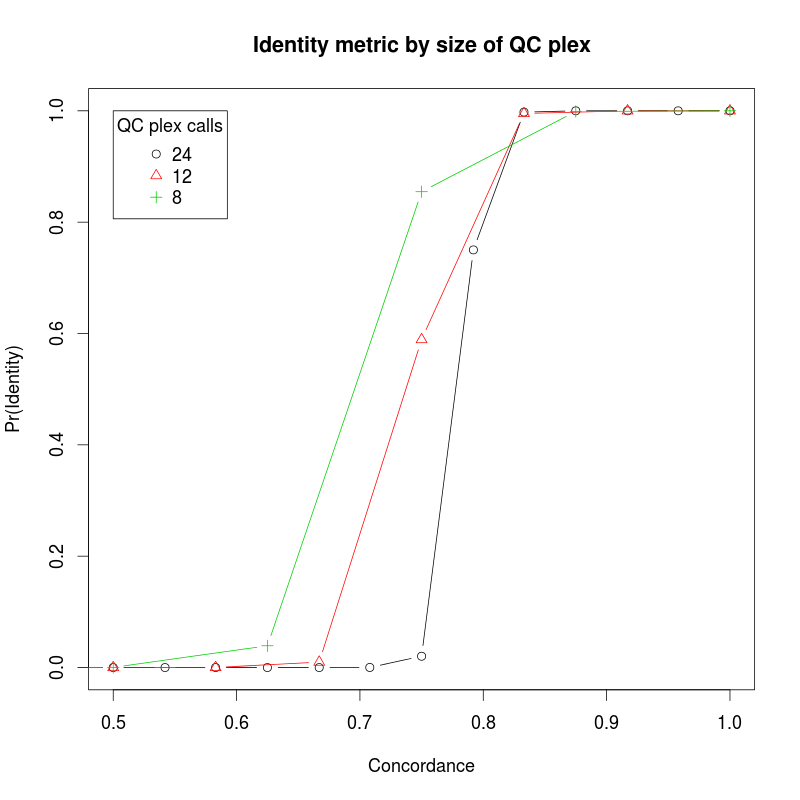
\includegraphics[scale=0.5]{identity_by_plex_size}

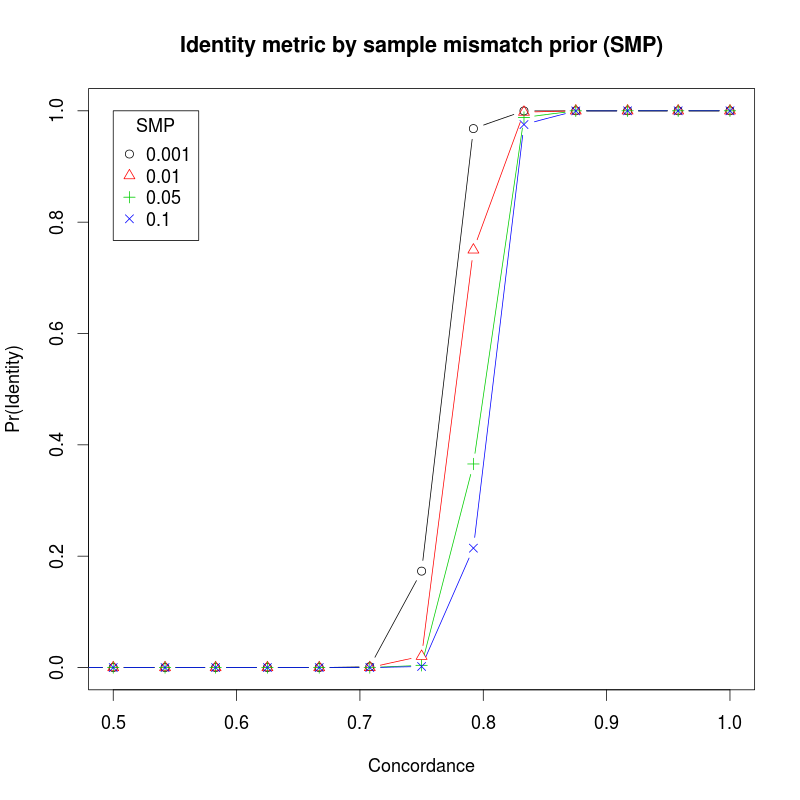
\includegraphics[scale=0.5]{identity_by_smp}

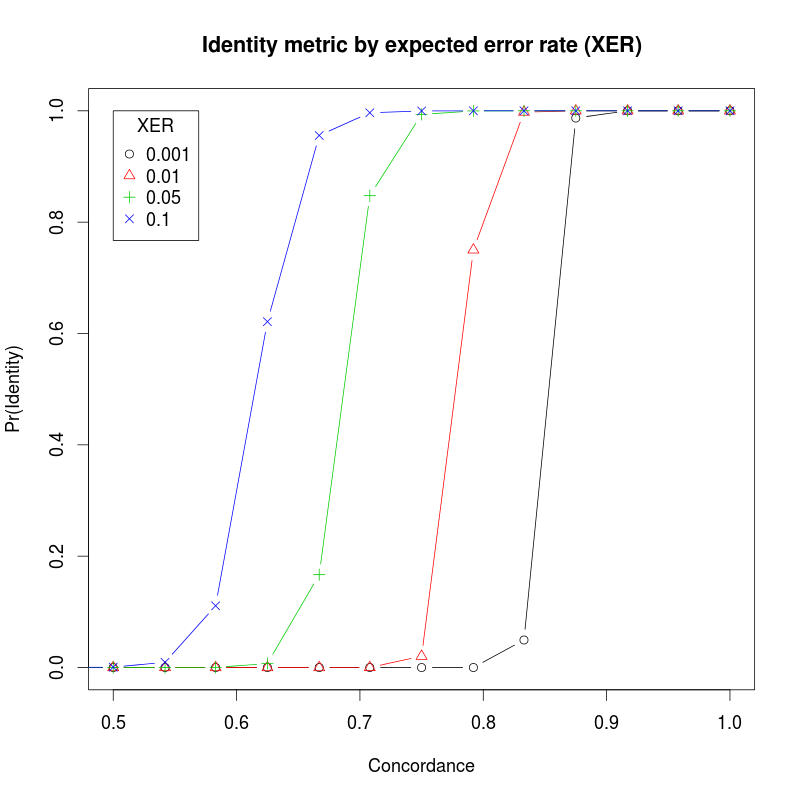
\includegraphics[scale=0.5]{identity_by_xer}

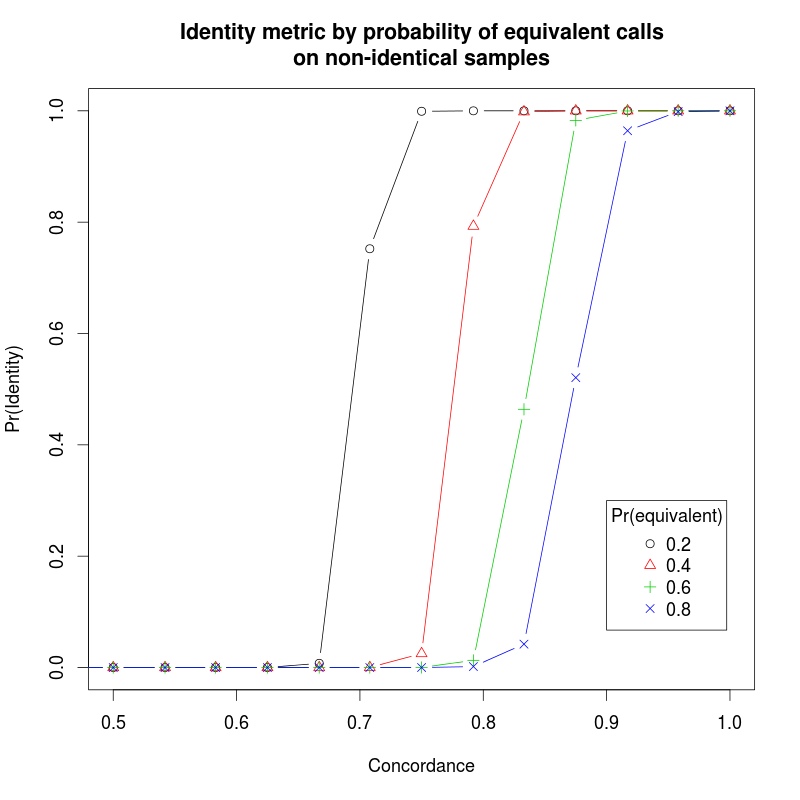
\includegraphics[scale=0.5]{identity_by_eq_prob.png}

\end{document}
